\chapter{Sprawdzenie poprawności wartości początkowych $U_{\textrm{PP}}$ oraz $Y_{\textrm{PP}}$}

Aby sprawdzić poprawność założonego punktu pracy, przyjęto, że sterowanie obietku na czas symulacji będzie stałe, równe $U_{\textrm{PP}}$. Po czasie ustalenia się odpowiedzi obiektu, zbadano wartość wyjścia oraz porównano ją z $Y_{\textrm{PP}}$.

\par Poniżej zamieszczono kod programu użytego do rozwiązania zadania:
\begin{lstlisting}[style=Matlab-editor]
%wyznaczanie y_pp dla u_pp = 1.1
u_pp = 1.1;

t_sim = 300;
y = [0;0];

for k=2:t_sim
    y_temp = symulacja_obiektu6Y(u_pp,u_pp,y(k),y(k-1));
    y = [y;y_temp];
end

y_pp = y(end);
\end{lstlisting}

Po ustalonym czasie symulacji \texttt{t\textunderscore sim = 300} zbadano przebieg sygnału wyjściowego.

\begin{figure}[h] 
\centering 
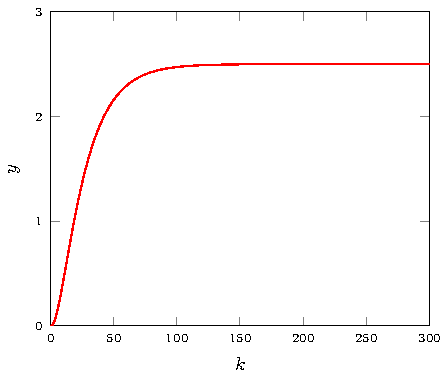
\includegraphics[scale=1.4]{wykresy/zad1_2/1_1.pdf} 
\caption{Odpowiedź układu dla ustalonego $u = U_{\textrm{PP}}$} 
\end{figure}

Wartość, na której ustalił się sygnał wyjściowy to \num{2.5}, co potwierdza poprawność założonego punktu pracy.